\documentclass[10pt,twocolumn]{style}
\usepackage{epsfig}
\title{Metric of Badness}
\author{Aydan R. Yumerefendi}

\begin{document}
  \maketitle

  \section{Binary Tree with Data at the Leaves}
  \label{sec:leaves}
  
  Let $T$ be a complete binary tree of height $h \geq 0$. We use $T$
  to aggregate data by suppling it to randomly chosen leaf nodes
  only; no internal tree node receives data directly. We assume that
  the probability of a node being malicious is independent of other
  nodes being malicious and is equal to $\epsilon$. Let $\alpha$ be
  the number of tree leaves that are either malicious or have a
  malicious parent. We will refer to $\alpha$ as the \emph{badness} of $T$
  and to the leaves that contribute to $\alpha$ as the
  \emph{suppressed} leaves of $T$.

  Let $X^k$ be a random variable equal to the number of suppressed leaf
  nodes in a tree of height $k \geq 0$. Let also $P(X^k_i)=P(X^k=i)$
  be the probability that there are $i$ suppressed leaf nodes. To
  compute $P(X^k_i)$ we make the following observations:
  \begin{enumerate}
    \item When {\bf $i<2^k$}, the root of the tree is not malicious.
    \item When {\bf $i=2^k$}, the root of the tree is malicious with
  probability $\epsilon$ and not malicious with probability
  $(1-\epsilon)$.
    \item When the root of the tree is not malicious, the desired
    probability can be computed by applying the same reasoning
    recursively to the left and right sub-trees.
  \end{enumerate}
  Taking all into consideration, we can express $P(X^k_i)$
  recursively as:
  \begin{eqnarray}\label{eqn:notmalicious}
    P(X^k_i) &=& (1-\epsilon)\sum_{j=0}^{j=i}P(X^{k-1}_j)P(X^{k-1}_{i-j})
    \textrm{, $i<2^k$}\\
    P(X^k_i) &=& \epsilon + (1-\epsilon)\sum_{j=0}^{j=i}P(X^{k-1}_j)P(X^{k-1}_{i-j})
    \textrm{, $i=2^k$}\\
     P(X^0_1)&=&\epsilon,P(X^0_0)=1-\epsilon, \textrm{ and }P(X^0_i)=0
    \textrm{, $i>1$}
  \end{eqnarray}

  On Figure~\ref{fig:distr} we plot the corresponding probability
  distribution for $h=9$ and $\epsilon=0.1$. The figure actually hides
  the mass at 512. This mass is several orders of magnitudes larger
  and is due to the probability of the root being malicious. This mass
  also explains the asymmetry in the shape of the distribution
  curve: the curve looks normal with some missing mass.

  \begin{figure}[htpb!]
    \begin{center}
      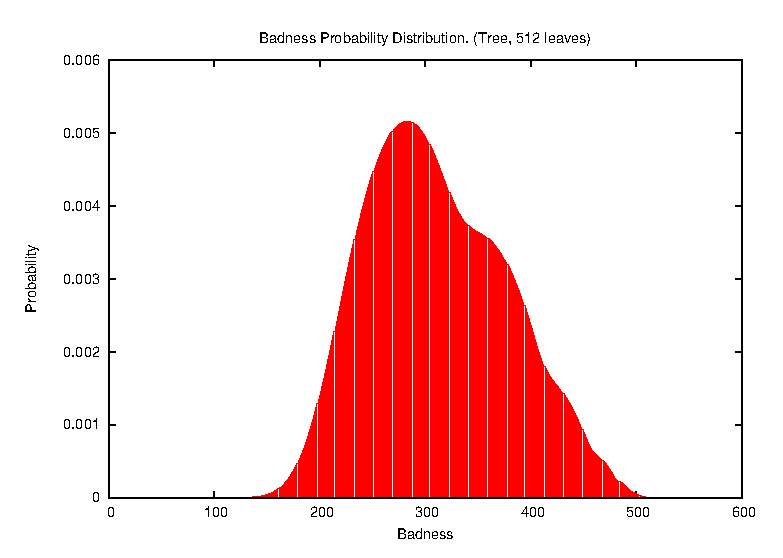
\epsfig{file=figs/badness,height=60mm}
      \caption{\label{fig:distr} Badness Probability Distribution for Binary Tree with
      512 leaves and malicious rate $\epsilon=0.1$. The mass at 512 is
      equal to 0.111111105770592 and is omitted from the graph.}
    \end{center}
  \end{figure}

  \section{Binary Tree with Data at all Nodes}
  \label{sec:nodes}
  Similarly to Section~\ref{sec:leaves}, let $T$ be a complete binary
  three of height $h \geq 0$. In this scenario instead of supplying data only to the
  leaves of $T$, we send a data value to any tree node. We use the
  same adversary model and define $\alpha$ to be the total number of
  tree nodes that are suppressed by the adversary: a suppressed node
  is either a malicious node, or a good node with a malicious parent.

  We can compute $P(X^k_i)$ in a similar manner:
  \begin{eqnarray}\label{eqn:notmalicious}
    P(X^k_i) &=& (1-\epsilon)\sum_{j=0}^{j=i}P(X^{k-1}_j)P(X^{k-1}_{i-j})
    \textrm{, $i<2^{k+1}-1$}\\
    P(X^k_i) &=& \epsilon \textrm{, $i=2^{k+1}-1$}\\
     P(X^0_1)&=&\epsilon,P(X^0_0)=1-\epsilon, \textrm{ and }P(X^0_i)=0
    \textrm{, $i>1$}
  \end{eqnarray}
  
  \begin{figure}[htpb!]
    \begin{center}
      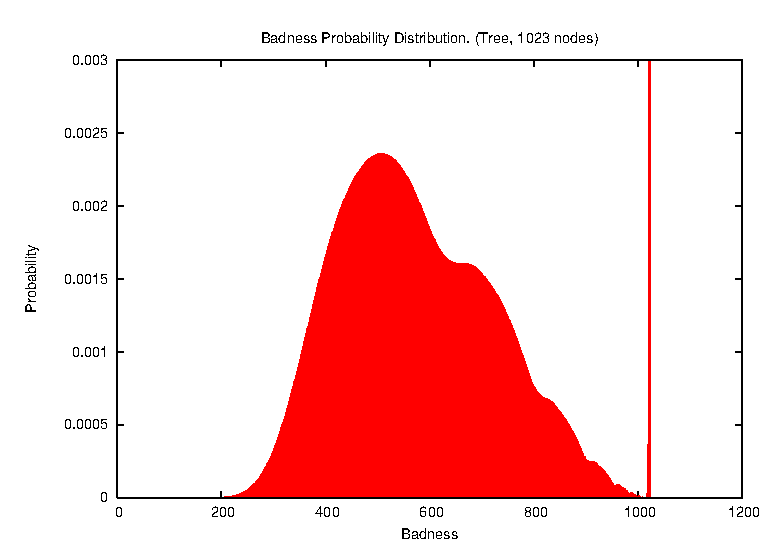
\epsfig{file=figs/badness_all,height=60mm}
      \caption{\label{fig:distr_all} Badness Probability Distribution for Binary Tree with
      1023 nodes and malicious rate $\epsilon=0.1$. The masses at 1022
      and 1023 are 0.009 and 0.1 respectively and are truncated in the
      graph.}
    \end{center}
  \end{figure}

  On Figure~\ref{fig:distr_all} we plot the probability distribution
  of a binary tree of height $9$ and malicious rate
  $\epsilon=0.1$. Similarly to the previous scenario, the graph
  exhibits some irregularities, due to the increased mass at the right
  end of the spectrum. We can intuitively explain this phenomenon
  taking into consideration that nodes closer to the root have the
  same rate of malice, but their impact increases with their
  height. This observation can justify approaches (e.g. sampling) that try to ensure
  that nodes closer to the root of the tree are malicious with smaller
  probability. 
  
  \section{Effect of Tree Degree}
  \label{sec:degree}
  We can extend the computation of the distribution of badness to a
  tree of degree $m$. The only differences, as compared to the binary
  case, are the different values for the boundaries ($m^h$ and
  $\frac{m^{h+1}-1}{m-1}$ instead of $2^h$ and $2^{h+1}-1$) and the
  breaking up of $i$ to $m$ sub-trees instead of two. However
  comparisons between tree aggregation structures of different degrees
  are not straightforward. For the same tree height, a ternary tree
  has significantly more nodes than a binary tree. For all practical
  purposes any comparison between aggregation structures should be done
  for trees with approximately the same number of tree nodes.

  To provide some kind of comparison among the behavior of trees of
  different degrees, we will use the expected fraction of badness as a
  basic measure.  Let $f^h_\alpha$ be the fraction of badness in a
  tree aggregation structure of height $h$. Depending on whether we
  use the approach of Section~\ref{sec:leaves} or
  Section~\ref{sec:nodes}, we can express $E[f^h_{\alpha}]$ as:\\
  
  {\bf Leaves}\\
  \begin{eqnarray}
    E[f^h_\alpha] = \epsilon + (1-\epsilon)E[f^{h-1}_\alpha]
  \end{eqnarray}

  {\bf Nodes}\\
  \begin{eqnarray}
    E[f^h_\alpha] = \epsilon + (1-\epsilon)E[f^{h-1}_\alpha]\frac{d^{h+1}-d}{d^{h+1}-1}
  \end{eqnarray}
  where $d$ is the tree degree.

  As we can see, $E[f^h_\alpha]$ is independent of the tree
  degree when we send data only to the tree leaves. When we send data
  to all tree nodes, we need to use a corrective factor to account for
  the difference in tree sizes. This corrective factor is less than
  1, and consequently the resulting expectation is smaller than the
  expectation when we send data only to the leaves (corrective factor
  of 1). This observation shows that sending data to the whole tree
  rather than to its leaves only reduces the expected fraction of
  badness. However, as the tree degree $d$ increases, the corrective
  factor becomes closer to 1 and consequently the expected fraction of
  badness increases. This phenomenon is due to the fact that as tree
  degree increases, the fraction of the leaves compared to the total
  number of tree nodes increases. Therefore, we can say that the
  expected fraction of badness sending data to the leaves only is an
  upper bound of the expected fraction of badness regardless of the
  method of dissemination. 


  %Using the observations from the previous paragraph, we can conclude
  %that using a binary aggregation tree in which we send data to all
  %tree nodes results in the smallest average fraction of badness. {\bf
  %It will be excellent if we can show that minimizing the expected
  %average fraction of badness will also minimize the other badness
  %moments, so that we can reason about the cases when we have
  %replication $c > 1$. But tests show that this is not the case}

  On Figure~\ref{fig:exp_badness} we plot the expected fraction of
  badness for trees of increasing height. We observe that as the tree
  height increases the expected fraction of badness increases as
  well. We can use this graph to reason about the security
  characteristics of trees of different degrees. Let $T_1$ and $T_2$
  be two complete trees with approximately the same number of nodes
  with degrees $d_1 < d_2$ and heights $h_1 > h_2$. Since $h_1 >
  h_2$, $E[f^{h_1}_{\alpha}] > E[f^{h_2}_{\alpha}]$. These
  inequalities show that the higher the tree degree, the smaller the expected level of
  badness. Consequently to minimize the expected level of badness, it
  is desirable to build trees of higher degrees. However, the higher
  the tree degree, the higher, the workload for an individual
  aggregator. Moreover, trees of higher degrees are harder to
  maintain in a distributed environment. 

  \begin{figure}[htpb!]
    \begin{center}
      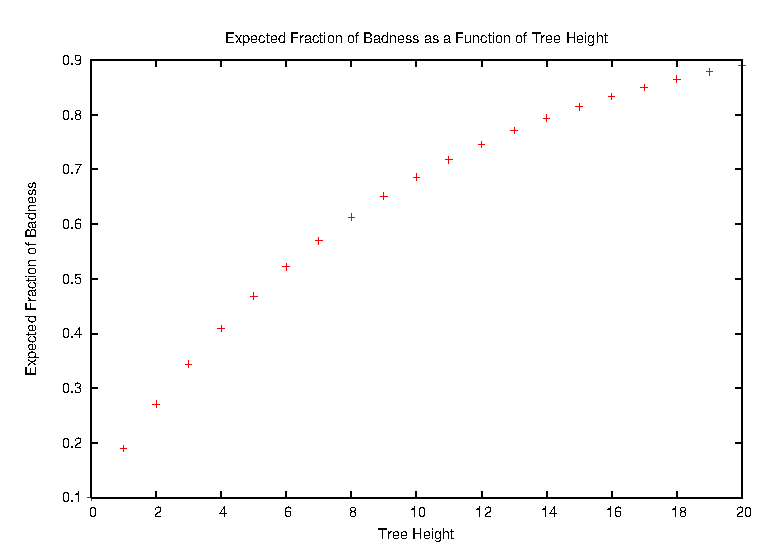
\epsfig{file=figs/expfrac.eps,height=60mm}
      \caption{\label{fig:exp_badness} Expected fraction of badness as a
      function of tree height.}
    \end{center}
  \end{figure}

  \section{Probability of Suppression}
  \label{sec:supress}
  We study the probability that no copy of a single value $v$ sent $c$ times to
  randomly chosen (with replacement) tree nodes is reported by the
  root of the tree. We will refer to this probability as the
  \emph{probability of suppression}. Let $A$ be the event that all $c$
  copies of $v$ are suppressed. Let $f_\alpha$ be the ratio of the
  level of badness to the total number of tree leaves
  (Section~\ref{sec:leaves}) or the total number of tree nodes
  (Section~\ref{sec:nodes}). Defined in this way $f_\alpha$ is equal
  to the probability that a single copy of $v$ is
  suppressed. Therefore, $P(A|\alpha)=f_{\alpha}^c$ and:
  \begin{eqnarray}
    P(A) = \sum_{\alpha=0}^{\alpha_{max}}f_{\alpha}^cP(\alpha)
  \end{eqnarray}
  where $\alpha_{max}$ is the maximum possible badness ($2^h$ for
  Section~\ref{sec:leaves}, and $2^{h+1}-1$ for Section~\ref{sec:nodes}).
  When $c=1$, we have that $P(A)=E[f_{\alpha}]$.

  \section{Effect of Tree Height}
  \label{sec:height}
  As tree height increases, the expected fraction of badness
  increases (Section~\ref{sec:degree}). We used this observation to
  justify the design decision of trying to construct shorter trees by
  increasing their degree. We can further decrease the expected
  fraction of badness by using multiple trees of smaller height. If
  the querier is willing to perform some additional amount of work, we
  can organize the existing aggregator nodes into multiple shorter
  trees and partition the data to be aggregated. The expected fraction
  of badness will be at most the expected fraction of badness of the
  tallest constructed tree.

  On Figure~\ref{fig:multiple_trees} we plot the expected fraction of
  badness for a scenario in which there are 4095 total aggregators
  with rate of malice $\epsilon=0.1$. 

  \begin{figure}[htpb!]
    \begin{center}
      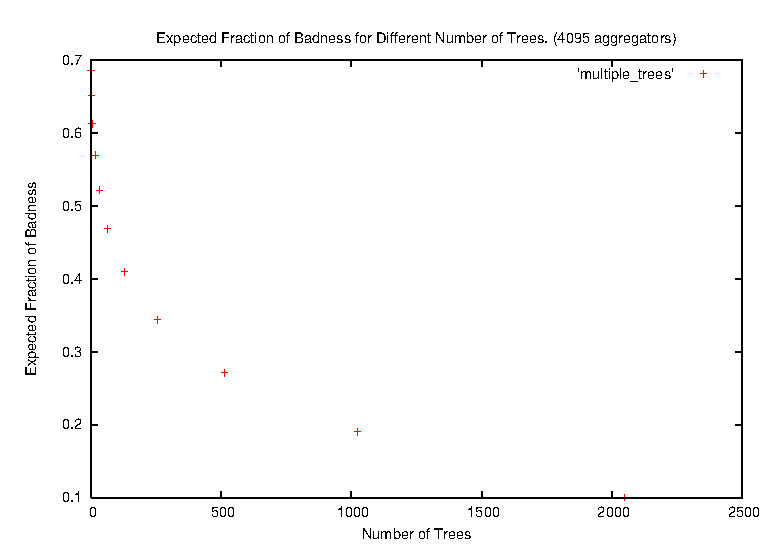
\epsfig{file=figs/multiple_trees,height=60mm}
      \caption{\label{sec:multiple_trees} Expected Fraction of Badness
      a Function of the Number of Aggregation Trees. Total number of
      aggregators 4095, $\epsilon=0.1$.}
    \end{center}
  \end{figure}

  \section{Effect of Replication}
  \label{sec:replicate}
  In Section~\ref{sec:supress} we derived a formula for the
  probability of suppression of a single value that is sent $c$ times
  to the aggregation structure. By increasing $c$, this probaility
  decreases, ands its complement (the probability of at least one copy
  not beight surpressed) increases. On Figure~\ref{fig:pb} we plot the
  complementary probability. we observe that 

  \begin{figure}[htpb!]
    \begin{center}
      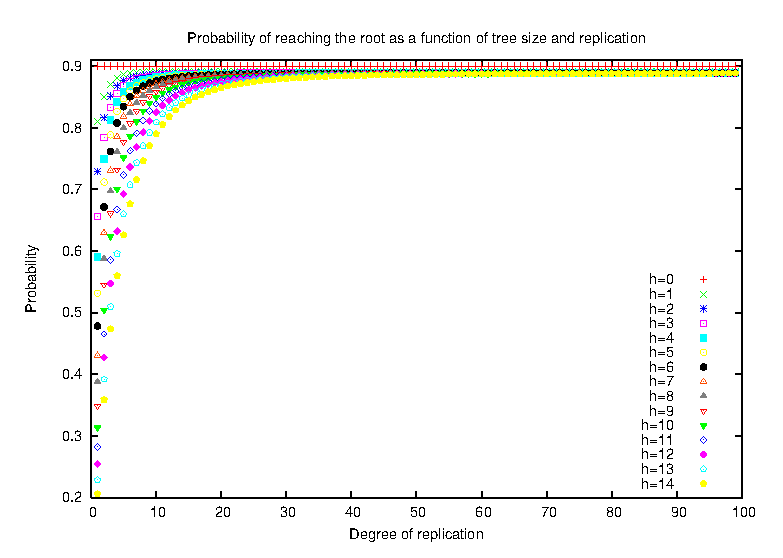
\epsfig{file=figs/tree_size,width=90mm}
      \caption{\label{fig:pb} Probability of at least one copy not
      being suppressed as a function of tree size and degree of
      replication. Rate of malice, $\epsilon=0.1$}
    \end{center}
  \end{figure}
  

  
  
%%   \section{Leaves vs. Nodes}
  
%%   where the initial factor of $(1-\epsilon)$ accounts for the fact
%%   that the root of the tree is not malicious.

%%   When $i=2^k$, the root will be malicious with probability $\epsilon$
%%   and not malicious with probability $(1-\epsilon)$. This case
%%   adds a small modification to Equation~\ref{eqn:notmalicious}:
%%   \begin{eqnarray}
%%     P(X^k_i) = \epsilon +
%%     (1-\epsilon)\sum_{j=0}^{j=i}P(X^{k-1}_j)P(X^{k-1}_{i-j})
%%     \textrm{, $i=2^k$} 
%%   \end{eqnarray}
%%   Finally, to terminate the recursive definition we have:
%%   \begin{eqnarray}
%%     P(X^0_1)=\epsilon,P(X^0_0)=1-\epsilon, \textrm{ and }P(X^0_i)=0
%%     \textrm{, $i>1$}
%%   \end{eqnarray}

%%   \begin{eqnarray}
%%     P(A) = \sum_{\alpha=0}^{\alpha=2^h}f_\alpha P(X^h_\alpha)
%%   \end{eqnarray}


%%   We can use $\alpha$ to estimate the probability that a value $v$ sent
%%   $c$ times to tree leaves chosen at random with replacement will be
%%   reported by the root of the tree. Let $A$ be the event that a single
%%   copy of $v$ does not get reported by the root. We have that $A$ occurs if and
%%   only if $v$ is sent to a suppressed leaf. Let $f_\alpha$ be the
%%   fraction of subverted leaves. We have that $P(A|\alpha)=f_\alpha$ and
%%   $P(\overline{A}|\alpha)=1-f_\alpha$. 

%%   Using the probability distribution, we can compute $P(A)$. We can
%%   even generalize to situations in which we send $c \geq 1$ copies of
%%   a value. Let $B$ be the event that when we send $c$ copies
%%   of the value to leaves chosen at random with replacement
%%   one of the copies is reported by the root. Clearly, $P(B|\alpha) =
%%   1-f_\alpha^c$ and therefore:
%%   \begin{eqnarray}
%%     P(B)=\sum_{\alpha=0}^{\alpha=2^h}(1-f_\alpha^c)P(X^h_\alpha)
%%   \end{eqnarray}


%%   On Figure~\ref{fig:pb} we plot $P(B)$ as a function of the
%%   aggregation tree size and the degree of replication. We observe that
%%   as the aggregation tree size increases, $P(B)$ decreases for the
%%   same values of $c$. This graph demonstrates an interesting property
%%   of aggregation trees: as the tree becomes taller, the probability of
%%   of data being suppressed increases. This is both a useful and
%%   intuitive observation: hierarchical aggregation increases the
%%   probability of suppression. We can exploit this fact to control the
%%   probability of suppression. If a querier is willing to do some part
%%   of the aggregation itself, then we can partition data among multiple smaller
%%   aggregation trees and decrease the probability of suppression.
  \section{Aggregation Bounds}
  
  {\bf Probability that a Min/Max is $k$ Positions Away from the
  Correct Min.}
  Let $X$ be a random variable describing the distance of the reported
  smallest/largest element from the true smallest/largest element. For
  a given level of badness, we have: $P(X=k|\alpha) = (f_{\alpha}^c)^k(1-f_{\alpha}^c)$. Accounting for all
  possible levels of badness:
  \begin{eqnarray}
    P(X=k)=\sum_{\alpha=0}^{2^h}(f_{\alpha}^c)^k(1-f_{\alpha}^c)P(\alpha)
  \end{eqnarray}
  For the expectation of $X$ we have:
  \begin{eqnarray}
    E[X] = \sum_{k=0}^{n-1}k\sum_{\alpha=0}^{2^h}(f_{\alpha}^c)^k(1-f_{\alpha}^c)P(\alpha)
  \end{eqnarray}
  where $n$ is the number of distinct elements.
%  When we condition by $\alpha$, $X$ has a modified geometric
%  distribution and $E[X|\alpha] =
%  \frac{f_{\alpha}^c}{1-f_{\alpha}^c}$. Therefore:  
%  \begin{eqnarray}
%    E[X] = \sum_{\alpha=0}^{\alpha=2^h}\frac{f_{\alpha}^c}{1-f_{\alpha}^c}P(\alpha)
%  \end{eqnarray}
%
%  {\bf Note:} This is not exactly the case: k does not go to infinity.
  
  {\bf Note:} While we can argue about the distance of the reported
  extreme value, it is impossible to argue about its difference in
  magnitude with respect to the actual extreme. Such analysis requires
  knowledge of the actual distribution of the data values.

  {\bf Probability that an FM zero position is $k$ smaller than the
  actual position.} A single FM bitvector has a structure similar to the one
  shown of Figure~\ref{fig:bitvector}. FM uses the position of the
  least significant zero bit to compute its estimate. An adversary can
  only decrease this position (See protection against increase (coming
  soon)). Let $l$ be the correct position of the least significant
  zero bit and $X$ be a random variable describing the position of the
  least significant zero. For $X$ to be equal to $k$ ($0\leq k \leq l$), all
  bits prior to $k$ need to be turned on. For each bit position smaller than $k$ there is at least one data
  value that turns on this bit, and on the average, if the bit's
  position is $i$, there are $2^{l-i}$ such values. We have:
  \begin{eqnarray}
    P(X=k) \geq \sum_{\alpha=0}^{2^h}(1-f_{\alpha}^c)^{k-1}P(\alpha)
  \end{eqnarray}

  For the expectation of $X$, we have:
  \begin{eqnarray}
    E[X] \geq \sum_{k=0}^{\log_2{n}}k\sum_{\alpha=0}^{2^h}(1-f_{\alpha}^c)^{k-1}P(\alpha)
  \end{eqnarray}



  

%  \begin{figure}[htpb!]
%    \begin{center}
%      
\epsfig{file=figs/bitvector,width=90mm,bbllx=12pt,bblly=12pt,bburx=311pt,bbury=41pt,clip=true}
%      \caption{\label{fig:bitvector} Structure of an FM bitvector.}
%    \end{center}
%  \end{figure}

\end{document}
